\section{Introduction}\label{intro}
Event-B~\cite{ABR10} is one of a number of formal methods that may be used to model systems where a high degree of reliability is required. Event-B was inspired by its predecessor, \emph{Classical-B}~\cite{TheBBook}. It is a modelling language, used with a supporting tool platform, Rodin~\cite{abrial10rodin}; so named from the project in which it was developed~\cite{RodinTool}. Further work was undertaken in the DEPLOY~\cite{DEPLOY} project to assess the approach with a number of the industrial partners. To derive the greatest benefit from the formal modelling approach, it is desirable to use the formal modelling artefacts to generate implementations for, at least, some parts of the system being modelled. During the latter stages of the DEPLOY project, automatic generation from Event-B models began to evolve, as the platform stabilized, where we targeted multi-tasking, embedded control systems. Initially, we chose Ada~\cite{ada2005} as a basis for our approach. This was not only because of it's suitability for the application domain, but also because the programming constructs are well-considered programming abstractions. Ada maps well to Event-B modelling elements, which is easy for modelling, and simplifies the translation to code. We do not attempt to model all aspects of the system, e.g. time; but we model the evolution of the system state, and are able to specify properties relating to the state, that are important for system safety. In current work, in the Advance project~\cite{advance}, we are concerned with modelling and co-simulation of Cyber-physical systems. We can, again, make use of automatic code-generation techniques to provide implementations for use in co-simulation.    


\subsection{Previous Work}
Initial development of the code-generation approach began from an object-oriented perspective, with the implementation-level notation, object-oriented, concurrent-B (OC-B)~\cite{Edmunds2009}. The focus of this work was to use Event-B  to model and generate code for safe multi-tasking with object-oriented languages. We initially targeted the Java~\cite{JavaSpec} language. We found, however, that this approach gave rise to a notation where the semantic gap between Event-B and the OC-B was quite large. This was not optimal for developers of Event-B models, who then wanted to write implementation-level specifications, from which code could be generated. We also found that models quickly became large and intractable; we recognized the need for decomposition of models into smaller units. At that time, Event-B tools were at an early stage of development, and machine decomposition was still in development. 

We decided to modify the approach, to use the newly developed decomposition approach~\cite{decomp2010c,decomp2010b}, and use an implementation-notation more closely related to Event-B (than OC-B, which was an object-oriented notation). The focus, then, became generating safe concurrent implementations, rather than targeting object-oriented technology, per se. This gave rise to our approach, known as Tasking Event-B. Our interest in safe, concurrent implementations drove us towards the Ada tasking model. At the implementation-level, an Event-B model is effectively a detailed model of an implementation. We found that the Ada~\cite{ada2005} programming language provides clearly defined constructs, that map well to Event-B, see Fig.~\ref{fig:B_Ada}. Ada tasks and protected objects can be modelled by Event-B machines in a one-one mapping. We distinguish between the two entities by annotating the machines with the AutoTask and Shared keywords. We describe the mapping in more detail in Sect.~\ref{tasks}.
%
\begin{figure}
\centering
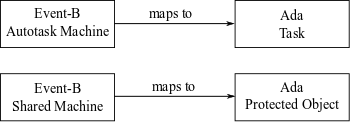
\includegraphics[width=0.5\textwidth]{graphics/B_Ada.png}
\caption{Mapping between Event-B and Ada}
\label{fig:B_Ada}
\end{figure}
%

In Sect.~\ref{eventb} we introduce the core Event-B features to the reader, and compare Event-B with some other formal approaches.  In Sect.~\ref{features} we provide an overview of some additional Event-B features required for code generation, and discuss some of the potential target programming language targets.

In Sect.~\ref{} we...
In Sect.~\ref{} we...

\section{Event-B Modelling}\label{eventb}
The formal methods related to the work presented here can be categorized as state-based formal methods. Alternative, but not unrelated, approaches are categorized as process-based methods. Classical-B~\cite{TheBBook,CNP,B4Free,atelierB} and its successor, Event-B are said to be state-based, since they focus on modelling the changes of state, not the behaviour of processes. In Classical-B, state updates are modelled by guarded operations, where the operation is an analogue of a procedure call in a programming language. In Event-B, state updates are modelled by guarded events, providing a more abstract view of the way a system evolves. Event-B can be used to model systems at an abstract level; and by adding more detail (using a technique called refinement) it can model the software aspects of systems too. Both methods are set theoretic modelling approaches that incorporate a notion of proof to show that important system properties are maintained. The former is primarily an approach to software systems development, the latter more widely applicable to system-modelling. In an effort to make modelling and proof easier, Event-B was developed to overcome some of the difficulties encountered when using in Classical-B. The main differences between Classical and Event-B are highlighted in~\cite{Hallerstede07}, and inspiration was also drawn from action systems~\cite{Back1990133}.

It is fair to say that Event-B is not just a formal modelling language; the name is used to describe both a notation, and a methodology. In addition to this a mature tool-platform called \emph{Rodin}, named after its development programme, complements the methodology. The main modelling components of Event-B are contexts and machines. Contexts are used to model static features using sets, constants, axioms, and theorems. Machines are used to model variable state using \emph{variables}. A third, more recent addition, is the Theory component; where a developer can augment the bundled mathematical language, and rule-base, with new (inference and re-write) rules, data types, and operators. During the modelling process, changes to the components result in automatic generation of proof obligations, which must be discharged in order to show that the development is consistent. The proof obligations generated in classical-B are often complex, the Event-B approach results in simpler proof obligations as described in~\cite{Hallerstede07}, since Event-B consists of a simplified action syntax, giving rise to simpler proof obligations. A further simplification was made by adopting an event-based approach, where each atomic event has a predicate guard and an action consisting only of assignment statements. Events correspond to operations in the B-method; operation specification was more expressive, and included constructs for specifying operation preconditions (as part of its Design by Contract approach), operation calls, return parameters, and more complex structures for branching and looping. These constructs are not features of Event-B. Due to these simplifications (and more efficient proof tools) a large number of the proof obligations may be discharged automatically, by the automatic provers. Where un-discharged proof obligations remain, the user has, at their disposal, an interactive prover. Various techniques can be applied, to discharge the proof obligations, such as adding hypotheses; or making use of the hyperlink-driven user interface, for rule and tactic application. In the early stages of development with Event-B, a developer will begin by abstracting, and modelling, the observable events occurring in a system. Event-B, as the name suggests, takes an event-based view of a system; where events occur spontaneously from the choice of enabled events. An event is said to be enabled when the guard is true, and the state updates, described in the event actions, can take place; otherwise it is disabled, and none of its updates can occur.  

\subsection{An Event-B Example}
An example of an Event-B machine can be seen in Fig.~\ref{fig:controllerSpec2}. It shows an abstract model of a pump controller, used in one of the case studies. We will use this model to describe some features of Event-B. But first we introduce the case study, which models a discrete \emph{pumpController}. The model describes a system where the controller receives a value for the level of fluid in a tank. The variable \emph{e\_level} represents the value in the environment, and \emph{c\_level} models the value at a port in the controller. The value at the port is stored internally in \emph{c\_level\_internal}. We adopt the prefix \emph{e\_} and \emph{c\_} throughout, to model environment and controller variables resp. and the suffix \emph{\_internal} to represent the controllers view of the environment. Reactive interactions between controller and environment are described as requests or commands. A Boolean value \emph{e\_pumponReq} represents an operator's request to turn the on pump. Based on the inputs to the controller, a command to turn the pump on may be issued, or a warning issued (and no command issued) if a minimum level \emph{MIN} is not satisfied.    
%
%
%
\begin{figure}[h]
\centering
\begin{minipage}{0.8\textwidth}
\textcolor{blue}{MACHINE} m2 \textcolor{blue}{REFINES} m1 \textcolor{blue}{SEES} ctx \\
\textcolor{blue}{VARIABLES} \text{c\_level, e\_level, c\_pumpOnReq, e\_pumpOnReq,} \hspace*{0.2cm} c\_pumpOnCmd, e\_pumpOnCmd, c\_warn, e\_warn,\\
\hspace*{0.2cm} c\_level\_internal, c\_pumpOnReq\_internal, c\_pumpOnCmd\_internal\\
\textcolor{blue}{INVARIANTS}\\
\hspace*{0.2cm}(c\_level\_internal $\leq$ MIN $\land$ c\_pumpOnReq\_internal = TRUE $\land$\\
\hspace*{0.5cm} commit = TRUE $\limp$ c\_warn\_internal = TRUE)\\
\hspace*{0.2cm} $\land$ (c\_level\_internal $>$  MIN $\land$  c\_pumpOnReq\_internal = TRUE $\land$\\
\hspace*{0.5cm} commit = TRUE $\limp$  c\_pumpOnCmd\_internal = TRUE)\\
\hspace*{0.2cm} $\land$ (c\_level\_internal $\in  \intg$)\\
\hspace*{0.2cm} $\land$ (c\_pumpOnReq\_internal $\in$  BOOL) \ldots\\
\textcolor{blue}{EVENTS}\\
\textcolor{blue}{INITIALISATION} c\_level :=  100 $\pprod$ e\_level := 90 $\pprod$ c\_pumpOnReq :=  FALSE $\pprod$ \ldots\\
\textcolor{blue}{EVENT} getLevel\_eAPI \textcolor{blue}{REFINES} getLevel\_eAPI\\
\hspace*{0.2cm}\textcolor{blue}{ANY} p1\\
\hspace*{0.2cm}\textcolor{blue}{WHERE} p1 = e\_level  \\
\hspace*{0.2cm}\textcolor{blue}{THEN} c\_level :=  p1\\
\hspace*{0.2cm}\textcolor{blue}{END}\\
\ldots
\end{minipage}
\caption{An Event-B  Pump Controller Model}
\label{fig:controllerSpec2}
\end{figure}
%
%
%
\begin{figure}[b]
\centering
\begin{minipage}{0.3\textwidth}
\textcolor{blue}{CONTEXT} ctx  \\
\textcolor{blue}{CONSTANTS} MIN\\
\textcolor{blue}{AXIOMS} MIN = 10
\end{minipage}
\caption{An Example Context}
\label{fig:context}
\end{figure}
%
%
 In Fig.~\ref{fig:controllerSpec2}, we see that machine \emph{M1} refines another machine \emph{M0}; we will discuss refinement in Subsect.~\ref{ref}. It also has a \emph{SEES} clause; this makes the contents of a context visible to a machine. Contexts may contain sets, constants, axioms and theorems, and example context can be seen in Fig.~\ref{fig:context}. There are variables representing the internal state of the controller, and invariants providing type information for variables. Invariants are also used to describe the safety properties of the system. This describes a required safety property, that if the level is at or below \emph{MIN}, and a user's pump-on request is detected, then a warning will be issued. Also, if the level is OK and a pump-on is requested, then the state \emph{pumpOnCmd = TRUE} is  set.  Following the \emph{INVARIANTS} clause are the model's \emph{Events}. The \emph{Initialisation} event is special event, since it has no guards. The initialisation event of a machine must occur before any other event in the machine is enabled. The event in the figure has a parameter \emph{p}, in the \emph{ANY} clause. Parameters can be used to represent information flow, in and out of events, or they can represent a \emph{local} variable within the scope of the event. The event guard is defined in the \emph{WHERE} clause, in the example, where \emph{p} is typed as a Boolean. The guard relates the parameter to a machine variable \emph{c\_pumpOnCmd}, in the predicate $ p = c\_compound$. The event action appears in the \emph{THEN} clause, where the parameter is assigned to the variable \emph{m\_pumpOnCmd}, in the expression $m\_pumpOnCmd := p$.


\subsection{Refinement and Extension}\label{ref}
As we mentioned earlier in the section, Event-B makes use of a technique called refinement, where a machine can be refined by another. Fig.~\ref{fig:refine} shows this relationship.
%
\begin{figure}
\centering
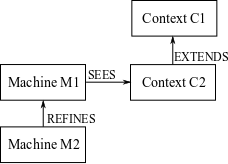
\includegraphics[width=0.5\textwidth]{graphics/refinement.png}
\caption{Refinement and Extension}
\label{fig:refine}
\end{figure}
%
%
The refined machine is augmented with state variables, events and invariants, to provide a more detailed specification satisfying the properties, specified in the invariants, of the abstract specification. The counterpart to refinement of machines, is extension of contexts. It is then possible to build upon pre-existing contexts, using the \emph{EXTENDS} clause, by adding more sets, constants, axioms and theorems. When a machine \emph{SEES} a context, the contexts that it extends are also accessible to the machine. In a refinement, new variables, events and invariant properties can be added. Existing events can be modified, but in a restricted manner. Machine refinement is transitive and leads to a hierarchical structure. Refinements are related to their more abstract counterparts in such a way that, a valid refinement always satisfies the specifications higher in the refinement hierarchy. In this way, important system properties can be specified at a high level of abstraction, and maintained down through the refinement chain. The Event-B tools are responsible for generating the proof obligations relating to refinement; these must be discharged in a similar way to those generated for proof of machine consistency. It is often necessary to specify a linking invariant, to describe the relationship between the variables of the abstract and refinement machines. Inspection of the proof obligations can assist in this task since some of the un-discharged proof obligations provide information about this link. In some cases we may model entities in an abstraction that are defined in the event parameters; and in the refinement these entities may be introduced to the model as machine variables. To assist with the proof effort we have a slightly different strategy to that of refining abstract variables with concrete variables. We link the parameters of the abstract event, with their concrete counterpart, using a $WITNESS$. This construct is a predicate describing the relationship between an event parameter (that disappears) from an abstract model, and the corresponding (refining) variable in the concrete model. Another feature of Event-B is the ability to  refine one atomic event with a number of events, thus breaking the atomicity, as described in~\cite{Butler08}. Eventually, at the end of a refinement chain the models are detailed enough to accurately describe an implementation. But Event-B is a modelling language, and there is a disjunction between the description of the system in Event-B, and commonly used programming languages, such as Java~\cite{JavaSpec}, C~\cite{KernighanR88} and Ada~\cite{ada2005}. Addressing the semantic gap between Event-B and programming constructs is a contribution of this article. 
%
